% =====================================================================
%  main.tex -- ARBITER / escalation-tax routing
%  CONFIDENTIAL. Patent filing pending. Do not circulate or submit.
%
%  DRAFT STATUS
%  ------------
%  Written by Claude as a first draft for Indrajeet and his mentor to
%  rewrite. Sections I--IV, VI-B and VII are drafted. Section V and
%  Sections VI-A and VI-C wait for the labelling and routing results.
%
%  TEMPLATE
%  --------
%  Official IEEE Access LaTeX template (ACCESS_latex_template_20260513,
%  from ieeeaccess.ieee.org). ieeeaccess.cls loads the bundled IEEEtran.cls.
%  Its fonts (.pfb, .tfm, .fd, .map), logos and spotcolor.sty stay in this
%  directory, because pdflatex looks for them next to main.tex. IEEE fills
%  in \history and \doi on acceptance.
%
%  MARKERS
%  -------
%  \tbd{...}          number or statement that depends on an unrun experiment
%  \citeneeded{...}   claim that needs a source not yet verified into refs.bib
%  \decision{...}     open decision from notes/experimental-protocol.md S12
%  \generated{f}{c}   float c, or a TBD marker while f is still ungenerated
% =====================================================================

\documentclass{ieeeaccess}

\usepackage{cite}
\usepackage{amsmath,amssymb,amsfonts}
\usepackage{graphicx}
\usepackage{textcomp}
\usepackage{booktabs}
\usepackage{multirow}
\usepackage{array}
\usepackage{tabularx}
\usepackage{xcolor}
\usepackage{url}

% Bold math in Times, as in the IEEE Access sample file.
\makeatletter
\AtBeginDocument{\DeclareMathVersion{bold}
\SetSymbolFont{operators}{bold}{T1}{times}{b}{n}
\SetSymbolFont{NewLetters}{bold}{T1}{times}{b}{it}
\SetMathAlphabet{\mathrm}{bold}{T1}{times}{b}{n}
\SetMathAlphabet{\mathit}{bold}{T1}{times}{b}{it}
\SetMathAlphabet{\mathbf}{bold}{T1}{times}{b}{n}
\SetMathAlphabet{\mathtt}{bold}{OT1}{pcr}{b}{n}
\SetSymbolFont{symbols}{bold}{OMS}{cmsy}{b}{n}
\renewcommand\boldmath{\@nomath\boldmath\mathversion{bold}}}
\makeatother

\newcommand{\tbd}[1]{\textcolor{red}{[TBD: #1]}}
\newcommand{\citeneeded}[1]{\textcolor{red}{[CITATION NEEDED: #1]}}
\newcommand{\decision}[1]{\textcolor{orange}{[DECISION: #1]}}
% \generated{file}{content}: typeset content once the analysis scripts have
% written file, and a marker until they have, so the draft always compiles.
\newcommand{\generated}[2]{\IfFileExists{#1}{#2}{\tbd{not yet generated:
\url{#1}}}}

% Notation used throughout
\newcommand{\cells}{\mathcal{C}}
\newcommand{\cstar}{c^{\star}}
\newcommand{\cost}{\kappa}
\newcommand{\Tax}{\mathrm{Tax}}
\newcommand{\Esc}{\mathrm{Esc}}
\newcommand{\Stk}{\mathrm{Stk}}
\DeclareMathOperator*{\argmin}{arg\,min}
\DeclareMathOperator*{\argmax}{arg\,max}

\begin{document}
\history{Draft for internal review, not for circulation. Date of publication
xxxx 00, 0000, date of current version xxxx 00, 0000.}
\doi{10.1109/ACCESS.2024.0429000}

\title{The Escalation Tax: One-Shot Selection of the Minimum Sufficient
Model Size and Reasoning Mode, with Router Cost Charged}

\author{\uppercase{Indrajeet Mondal}\authorrefmark{1}
\decision{mentor co-authorship and author order; IEEE membership; ORCID
iDs}}

\address[1]{\decision{department, institution, city and postal code,
country; e-mail}}
\tfootnote{\decision{funding statement, or remove}}

\markboth
{I. Mondal: The Escalation Tax}
{I. Mondal: The Escalation Tax}

\corresp{Corresponding author: Indrajeet Mondal
(e-mail: \decision{corresponding-author e-mail}).}

\begin{abstract}
Tiered language-model services leave the user to choose both a model size
and, increasingly, whether the model should reason before answering. Users
misallocate in two opposite directions. They start small and escalate after
each failure, paying in full for every discarded attempt and for resending
the prompt, or they leave a heavyweight configuration selected and pay a
premium on prompts that never needed it. We call the resulting excess over
the cheapest configuration that would have succeeded the \emph{escalation
tax}, formalise it, and decompose it into an escalation component and a
stickiness component. We then ask whether a small predictor, placed in
front of an eight-cell pool of Qwen3 models (0.6 to 8 billion parameters,
each with thinking on and off), can select that minimum sufficient
configuration before any generation, and whether the saving survives once
the router is charged for its own tokens, latency and energy. Every prompt
in a stratified corpus of mathematics, code, multiple-choice and open-ended
tasks is run through all eight cells on a consumer laptop graphics card
with measured board power. We compare classical classifiers, fine-tuned
encoders and a small language model used as a router against manual
escalation policies and a self-verifying cascade. The tax is then measured
on two pools the laptop cannot host: thirteen public models priced by their
providers, and six hosted cells in which reasoning effort is a paid
setting. \tbd{headline tax, net saving of the best router, energy per
solved query, and the router-family ordering once charged}.
\end{abstract}

\begin{keywords}
Energy efficiency, hybrid thinking, inference cost, large language models,
model routing, reasoning effort, test-time compute.
\end{keywords}

\titlepgskip=-21pt

\maketitle

% =====================================================================
%  I. INTRODUCTION
% =====================================================================
\section{Introduction}
\label{sec:introduction}

\IEEEPARstart{A}{nyone} who uses a tiered language-model service makes an
allocation decision before typing a word. Providers sell families of models
that trade capability against price and latency, and a growing number also
expose a second control: whether, and how much, the model should reason
before it answers~\cite{openai_reasoning,anthropic_effort,google_thinking}.
Open-weight families
now ship the same two axes. Qwen3 offers dense models from 0.6B to 14B
parameters with a switch between thinking and non-thinking modes and a
controllable thinking budget~\cite{qwen3}. Reasoning traces raise accuracy
on hard problems~\cite{wei2022cot,deepseek2025r1}, but they multiply the
number of generated tokens, and the choice of when to pay for them is left
to the person holding the keyboard.

People get that choice wrong in two opposite directions. The first is
under-provisioning: start with a small, cheap configuration, notice a wrong
answer, and move up. Every failed attempt is billed in full, and so is the
prompt, which has to be resent at each step. The second is
over-provisioning. A heavyweight configuration chosen for yesterday's hard
task stays selected, and today's trivial prompts pay its premium. Reasoning
models make the second failure worse because they tend to produce long
traces for questions that need none, a pattern the efficient-reasoning
literature calls overthinking~\cite{sui2025stopoverthinking,
alomrani2025reasoningbudget}. Both failures waste tokens, time and energy,
and neither has been measured against the configuration that would have
been sufficient.

Model routing is the obvious remedy, and there is a large literature on
it~\cite{moslem2026routingsurvey}. Cascades query models in order of cost
and stop when a scorer accepts an answer~\cite{chen2023frugalgpt,
aggarwal2024automix}. Predictive routers pick a model from the query
alone~\cite{ding2024hybridllm,ong2024routellm}. More recent work routes over
reasoning mode~\cite{zhang2025synapseroute,lee2026dart} and over model and
reasoning strategy jointly~\cite{pan2026routetoreason}. These systems are
evaluated against static single-model policies, random assignment, an
oracle, or an automated cascade. None of the work we located evaluates
them against the policy people actually follow, which is manual escalation
with the prompt resent at every step. Energy-aware routers do measure power,
but they route over model choice or processing pipeline rather than
reasoning mode, and they report savings gross of the router's own
consumption~\cite{ziller2026greenserv,li2026ecothink}. Routers that control
reasoning effort report tokens and latency, not
joules~\cite{lee2026dart}.

This paper studies one-shot selection of the \emph{minimum sufficient
configuration}: the cheapest cell of a model-size by reasoning-mode grid
that still answers a prompt correctly, predicted before any generation. We
define the \emph{escalation tax} as the cost a policy incurs beyond that
configuration, and we split it into an escalation component, paid for
attempts that failed, and a stickiness component, paid for finishing on a
configuration more expensive than necessary. The study runs on hardware
that most practitioners own: a laptop with an 8\,GB consumer GPU, where
quantisation is forced, only one model fits in memory at a time, and every
joule is measured from board power rather than estimated from rated power.

The contributions are as follows.
\begin{itemize}
  \item A formal definition of the escalation tax and its decomposition,
        together with a family of manual escalation policies evaluated under
        both perfect and imperfect failure detection
        (Section~\ref{sec:methodology}).
  \item An oracle-labelled corpus in which every prompt is run through all
        eight cells of a Qwen3 size-by-mode grid, recording per-cell
        success, token counts, latency and measured energy
        (Section~\ref{sec:experimentation}).
  \item A comparison of three router families---classical classifiers,
        fine-tuned encoders, and a small language model used as a
        router---under \emph{net} accounting, in which each router's own
        tokens, latency and energy are subtracted from the saving it
        produces.
  \item A measured characterisation of the energy cost of the reasoning-mode
        axis, reported as joules per \emph{solved} query so that a cheap
        configuration that fails and forces a retry is not flattered.
  \item The same tax measured on two pools the laptop cannot host:
        thirteen public models priced by their providers, and six hosted
        cells in which reasoning effort is a paid setting, so the result is
        reported at frontier scale as well as on local hardware
        (Section~\ref{sec:results}).
  \item Two validation results that other studies on similar hardware can
        reuse: an empirical test of whether thinking and non-thinking modes
        are separate operating points at every model size, and evidence that
        a supported, monotonic NVML energy counter can nonetheless be
        non-physical on laptop GPUs.
\end{itemize}

The tax is large, and most of it comes from where a user stays rather than
how they climb. Leaving the 8B thinking cell selected pays 12.96 times the
minimum sufficient energy and answers 79.8\% of prompts; a frugal climb with
thinking off pays 0.89 times and answers 92.2\%. On these gradable tasks,
moving up a size below 8B without thinking answers more prompts than turning
thinking on, for 3.8 to 5.5 times less energy per solved prompt; on
open-ended requests, graded by a model judge that agrees with a human only
moderately, thinking is far cheaper, yet the frugal climb still pays the
least tax. How a router compares with that climb turns on how a failed route
is recovered. Sent to the largest cell, the best router spends 1.30 times
the climb's energy per solved prompt, though 64\% less than the sticky
default; recovering by climbing from the routed cell instead, every router
comes within 6\% of the climb and four are cheaper than it. Detection
matters as much: when users accept 15\% of wrong answers, the router answers
7.1 points more than the climb, because it makes fewer attempts at which to
be fooled.

The rest of the paper is organised as follows. Section~\ref{sec:literature}
surveys routing, reasoning-effort control and energy measurement for
language-model inference. Section~\ref{sec:methodology} formalises the
escalation tax and describes the routers and the cost model.
Section~\ref{sec:experimentation} gives the experimental setup, including
the corpus, labelling procedure, baselines, metrics and the two validation
gates. Sections~\ref{sec:results} and~\ref{sec:discussion} present and
interpret the results, Section~\ref{sec:future} outlines future work, and
Section~\ref{sec:conclusion} concludes.

% =====================================================================
%  II. LITERATURE SURVEY
%  Every factual claim about prior work below is taken from
%  notes/prior-art-register.md, which records what was verified and from
%  which source. Do not add a claim about a paper that is not in the
%  register without reading the paper first.
% =====================================================================
\section{Literature Survey}
\label{sec:literature}

The problem sits where three bodies of work meet: routing and cascading
across language models, control of reasoning effort at inference time, and
measurement of the energy that inference consumes. We review each, then
the small set of papers that combine two of them, and close with the gap
this study addresses.

\subsection{Routing and Cascading Across Models}
\label{sec:lit-routing}

The word \emph{routing} has two meanings in this area, and they should be
kept apart. Mixture-of-experts architectures route tokens between expert
sub-networks inside a single model~\cite{fedus2022switch}. This paper is
concerned with the other meaning: routing whole queries between separate
models, each of which could answer on its own. Moslem and Kelleher survey
that literature and organise it into routing, which commits to one model
before generation, and cascading, which tries models in
sequence~\cite{moslem2026routingsurvey}.

\emph{Cascades.} FrugalGPT sends a query through a sequence of models of
increasing price and stops when a learned scorer judges the answer
acceptable; its authors report matching the best individual model with up
to 98\% lower cost~\cite{chen2023frugalgpt}. AutoMix replaces the external
scorer with few-shot self-verification by the small model and decides
whether to escalate with a partially observable Markov decision process,
reporting cost reductions above 50\%~\cite{aggarwal2024automix}. AutoMix is
the closest published idea to the question asked here, because it treats
escalation as a sequential decision. Its decision state, however, is the
model's confidence in its own answer, not the cost already spent on failed
attempts, and it is an automated policy rather than a model of what a user
does. Both cascades share a structural cost: the cheap model must generate
before the system can decide, so every escalated query pays for at least one
discarded answer.

\emph{Predictive routers.} Hybrid LLM trains a router that estimates, from
the query alone, whether a small model's answer will be close in quality to
a large model's, and exposes a threshold that trades quality for cost at
test time, reporting 40\% fewer calls to the large model with no loss in
response quality~\cite{ding2024hybridllm}. RouteLLM learns a
strong-versus-weak decision from human preference data and reports more than
a twofold cost reduction~\cite{ong2024routellm}. RouterDC trains a query
encoder with dual contrastive losses so that queries sit near the models
that answer them well~\cite{chen2024routerdc}. UniRoute addresses the
practical problem that the model pool changes, routing to models unseen
during training and giving an excess-risk bound for the
procedure~\cite{jitkrittum2025universal}. Arch-Router instead aligns a
1.5B-parameter router with user-defined domain and action preferences so
that models can be added without retraining~\cite{tran2025archrouter}, and
Router-R1 moves to multi-round routing, training a model with reinforcement
learning to interleave its own deliberation with calls to other models and
to aggregate their outputs across rounds~\cite{zhang2025routerr1}.

\emph{Benchmarks.} Three benchmarks make routers comparable. RouterBench
provides a 36{,}497-prompt zero-shot split with outputs and per-inference
costs for 11 models, and oracle labels for the best model per
prompt~\cite{hu2024routerbench}. RouterEval scales the candidate pool to
more than 8{,}500 models and 200 million performance
records~\cite{huang2025routereval}. LLMRouterBench collects more than
400{,}000 instances over 21 datasets and 33 models, with code and data
released publicly~\cite{li2026llmrouterbench}.

Across this body of work, cost is denominated in API price, model calls or
tokens, and the comparison points are static single-model policies, random
assignment, an oracle, or another automated router or cascade.

\subsection{Reasoning Effort and Test-Time Compute}
\label{sec:lit-reasoning}

Chain-of-thought prompting showed that asking a model to write intermediate
steps improves multi-step reasoning~\cite{wei2022cot}, and self-consistency
improved it further by sampling several reasoning paths and taking a
majority vote over their answers~\cite{wang2023selfconsistency}. Both buy
accuracy with generated tokens. Reinforcement learning has since been used
to train models that produce long reasoning traces without being
prompted to~\cite{deepseek2025r1}, and simple interventions at decoding time
can lengthen or cut those traces: s1 introduced budget forcing, which ends
the thinking phase early or suppresses its end to extend
it~\cite{muennighoff2025s1}. Qwen3 builds the control into the model,
serving thinking and non-thinking behaviour from one set of weights with a
user-settable thinking budget~\cite{qwen3}.

Long traces are not always useful. Sui \emph{et al.} survey methods for
efficient reasoning and document the tendency of reasoning models to spend
many tokens on easy questions~\cite{sui2025stopoverthinking}. Alomrani
\emph{et al.} organise adaptive test-time compute into two tiers:
controllability under a fixed budget, and adaptiveness, where the budget
itself depends on the input~\cite{alomrani2025reasoningbudget}. Selecting a
reasoning mode per prompt is an instance of the second tier.

\subsection{Routing Over Reasoning Mode}
\label{sec:lit-mode-routing}

A recent group of papers routes over whether and how much to think, usually
within a single model. SynapseRoute trains a logistic-regression classifier
on query embeddings to send medical questions to thinking or non-thinking
mode of one dual-state model, reporting 36.8\% lower inference time, 39.66\%
fewer tokens and that about 58\% of the questions need no reasoning
mode~\cite{zhang2025synapseroute}. Think When Needed attaches a
lightweight router head that chooses Think or Non-Think before generation
for ranking tasks~\cite{guo2026thinkwhenneeded}. DART is training-free: it
generates two cheap non-thinking drafts, reads problem difficulty from their
agreement, and sets a per-query thinking budget accordingly, cutting
thinking tokens by 32--73\%~\cite{lee2026dart}. Learning When to Think moves
the decision inside the model, which emits NoThink, Short or Long as its
first token after training with GRPO~\cite{kassenaar2026learningwhentothink}.
HRBench compares prompt-based, external-routing and speculative switching
strategies across four training regimes, six models and five benchmarks, and
concludes that the preferred strategy depends on model scale and task
domain~\cite{ning2026hrbench}.

Route to Reason is the closest prior work to the grid studied here. It
selects jointly among seven open-source models and four reasoning strategies
under a budget constraint and reports more than 60\% fewer
tokens~\cite{pan2026routetoreason}. Its existence means that joint selection
of model and reasoning effort is not, by itself, a new idea, and we do not
claim it as one.

All of these papers depend on an assumption that is rarely tested: that a
model's thinking and non-thinking modes are genuinely different operating
points. Wang \emph{et al.} examined hybrid-thinking models directly and found
only partial separation, with reasoning behaviour leaking into non-thinking
outputs; their improved training recipe reduced non-thinking output length on
MATH500 from 1{,}085 to 585 tokens, a large gain that still falls short of
clean separation~\cite{wang2025demystifying}. A routing study whose grid
includes a reasoning-mode axis inherits this risk, which is why we test
separation on our own checkpoints before labelling
(Section~\ref{sec:gate-mode}).

\subsection{Energy and Carbon of Language-Model Inference}
\label{sec:lit-energy}

Strubell \emph{et al.} brought the energy and financial cost of training NLP
models to the field's attention~\cite{strubell2019energy}, and Schwartz
\emph{et al.} argued that efficiency should be reported alongside accuracy
as a first-class result~\cite{schwartz2020greenai}. Lacoste \emph{et al.}
provided a calculator for converting compute into emissions using regional
grid intensity~\cite{lacoste2019quantifying}, and Patterson \emph{et al.}
showed how strongly the emissions of large training runs depend on
hardware, data-centre efficiency and location~\cite{patterson2021carbon}.
For inference, Luccioni \emph{et al.} measured energy and carbon per
1{,}000 queries across task types and found wide variation between
them~\cite{luccioni2024powerhungry}.

Work on constrained hardware is closer to our setting. Camel reduces energy
on an NVIDIA Jetson AGX Orin by tuning GPU frequency and batch size for a
single model~\cite{xu2025camel}, and serving systems such as vLLM raise
throughput by managing key--value cache memory more
efficiently~\cite{kwon2023vllm}. Both are orthogonal to routing: they make
each configuration cheaper to run but do not decide which configuration to
run.

\subsection{Energy-Aware and Latency-Aware Routers}
\label{sec:lit-energy-routing}

Three routers treat energy or latency as part of the objective, and we read
each in full because they bear most directly on our claims. GreenServ routes
queries among 16 open models using task type, semantic cluster and text
complexity, measures GPU energy on an A100 with the Zeus library, and reports
a 31\% cumulative energy reduction with 22\% higher accuracy than random
routing~\cite{ziller2026greenserv}. It characterises its router's overhead
at about 7.77\,ms per query but does not subtract the router's energy from
the saving. EcoThink sends each query either to a retrieval path or to a
reasoning path using a distilled DistilBERT classifier, and reports a 40.4\%
average energy reduction across nine benchmarks and carbon of
1.32\,gCO$_2$e per query against 4.52 for GPT-4o~\cite{li2026ecothink}. Its
energy comes from CodeCarbon sampling combined with an average utilisation
of thermal design power, so it is partly estimated, and the router's own
cost is not charged. Yang \emph{et al.} route queries among edge experts on
RTX~4090 GPUs using two DistilBERT-based predictors and an actor--critic
policy, and optimise quality of service and latency without measuring
energy~\cite{yang2025qosrouting}.

Two observations follow. First, energy-aware routing is established, and so
is reporting carbon for it; neither is a contribution of this paper. Second,
these routers select a model or a pipeline. None of them routes over
reasoning mode inside a hybrid model, and none subtracts the router's own
measured energy from the energy it saves.

\subsection{Evaluation With Language-Model Judges}
\label{sec:lit-judges}

Open-ended prompts cannot be graded by string match, so routing studies that
include them rely on model judges. Zheng \emph{et al.} found that a strong
judge agreed with human preferences at a rate comparable to agreement between
humans, while also documenting position, verbosity and self-enhancement
biases~\cite{zheng2023judging}. The biases matter here because a judge drawn
from the same family as the routed models could favour them, which motivates
the out-of-family judge and the two-sided validation in
Section~\ref{sec:judge}.

\subsection{Positioning}
\label{sec:lit-gap}

Table~\ref{tab:prior-work} summarises the systems closest to this study.
Reading them together, four questions remain open in the literature we
located.

\begin{enumerate}
  \item \emph{The escalation tax is unmeasured.} Routers and cascades are
        compared with static, random, oracle or automated baselines. None
        formalises manual escalation, in which each failed attempt is billed
        in full and the prompt is resent to the next configuration.
  \item \emph{Router energy is not netted out.} Energy-aware routers report
        gross savings. We found no study that subtracts the selector's own
        measured energy, or that asks at what point a language-model router
        stops paying for itself against a linear classifier.
  \item \emph{The reasoning-mode axis has no measured energy cost.} Routers
        over reasoning mode report tokens and latency; routers that measure
        energy do not route over reasoning mode.
  \item \emph{Energy is not normalised by success.} Energy per query and per
        token are standard. Energy per \emph{solved} query, which charges a
        cheap failure for the retry it causes, was not found.
\end{enumerate}

\noindent The study also characterises the grid on an 8\,GB laptop GPU. That
is a useful regime to report, since the energy-aware routers above ran on
A100 and RTX~4090 hardware, but we treat it as context rather than as a
contribution in its own right.

% Table cells are drawn from notes/prior-art-register.md. Every row now
% agrees with the prose above, which states each system's own reported
% figures. Two rows were checked against the full texts because the prose
% did not pin the metric down: Router-R1's cost reward is output tokens
% weighted by a function of parameter count, and the QoS router's headline
% is a composite of quality and latency compliance rather than latency
% alone. The four 2023--2024 rows are long-established. Rows still worth a
% PDF pass before submission: SynapseRoute, DART, Learning When to Think
% and Route to Reason, whose decision points come from their abstracts.
\begin{table*}[!t]
\centering
\caption{Systems closest to this study. \emph{Axis} is what the router
selects; \emph{decision point} is when it commits; \emph{efficiency
reported} is the cost measure used in the headline result.}
\label{tab:prior-work}
\renewcommand{\arraystretch}{1.15}
\begin{tabularx}{\textwidth}{@{}l l >{\raggedright\arraybackslash}X >{\raggedright\arraybackslash}X@{}}
\toprule
System & Axis & Decision point & Efficiency reported \\
\midrule
FrugalGPT~\cite{chen2023frugalgpt} & Model & Cascade, scorer after each answer & API cost \\
AutoMix~\cite{aggarwal2024automix} & Model & Cascade, self-verification & Cost \\
Hybrid LLM~\cite{ding2024hybridllm} & Model (small/large) & Before generation & Large-model calls \\
RouteLLM~\cite{ong2024routellm} & Model (strong/weak) & Before generation & Cost \\
Router-R1~\cite{zhang2025routerr1} & Model & Multi-round & Parameter-weighted output tokens \\
SynapseRoute~\cite{zhang2025synapseroute} & Reasoning mode & Before generation & Tokens, time \\
DART~\cite{lee2026dart} & Thinking budget & After two short drafts & Tokens, latency \\
Learning When to Think~\cite{kassenaar2026learningwhentothink} & Thinking level & In-model, first token & Response length \\
Route to Reason~\cite{pan2026routetoreason} & Model and strategy & Before generation & Tokens \\
GreenServ~\cite{ziller2026greenserv} & Model & Before generation & Measured energy (gross) \\
EcoThink~\cite{li2026ecothink} & Retrieval or reasoning path & Before generation & Partly estimated energy, carbon (gross) \\
QoS edge routing~\cite{yang2025qosrouting} & Edge expert & Before generation & QoS score under a latency bound \\
\midrule
This study & Model size and reasoning mode & Before generation & Tokens, latency, measured energy (net of router) \\
\bottomrule
\end{tabularx}
\end{table*}

% =====================================================================
%  III. METHODOLOGY
%  Source: notes/experimental-protocol.md, sections 2, 3, 6, 7 and 8.
%  Where this text goes beyond the protocol, a comment says so.
% =====================================================================
\section{Methodology}
\label{sec:methodology}

\subsection{Configuration Grid}
\label{sec:grid}

The routed pool is a grid, not a ladder. It crosses four model sizes with
two reasoning modes, giving eight cells
$\cells = \{c_1, \dots, c_8\}$ (Table~\ref{tab:grid}). All cells come from
one model family, Qwen3, which offers a size ladder in which every model can
run with or without a thinking phase~\cite{qwen3}. Using one family means
that size and mode are the only things that vary between cells: tokenizer,
training recipe and chat template stay the same. Quantisation is held fixed
at 4-bit (Q4\_K\_M) for the same reason. The cost of that choice is that
results describe quantised models, a limitation we return to in
Section~\ref{sec:discussion}.

\begin{table}[!t]
\centering
\caption{The eight-cell configuration grid. Sizes on disk are for the
Q4\_K\_M weights used in all experiments.}
\label{tab:grid}
\renewcommand{\arraystretch}{1.1}
\begin{tabular}{@{}c l l r@{}}
\toprule
Cell & Model & Mode & Weights \\
\midrule
$c_1$ & Qwen3-0.6B & no-think & 0.52\,GB \\
$c_2$ & Qwen3-0.6B & think    & 0.52\,GB \\
$c_3$ & Qwen3-1.7B & no-think & 1.36\,GB \\
$c_4$ & Qwen3-1.7B & think    & 1.36\,GB \\
$c_5$ & Qwen3-4B   & no-think & 2.62\,GB \\
$c_6$ & Qwen3-4B   & think    & 2.62\,GB \\
$c_7$ & Qwen3-8B   & no-think & 5.23\,GB \\
$c_8$ & Qwen3-8B   & think    & 5.23\,GB \\
\bottomrule
\end{tabular}
\end{table}

\subsection{Cost of a Configuration}
\label{sec:cost}

We do not assume that cells are ordered by parameter count. A thinking cell
of one size can cost more than a non-thinking cell of the next size up, and
whether it does depends on the prompt. Cost is therefore measured per
prompt $q$ and per cell $c$, in three units:
\begin{align}
  \cost_{\mathrm{tok}}(c, q) &= \alpha\, n_{\mathrm{in}}(c, q)
                              + \beta\, n_{\mathrm{out}}(c, q),
  \label{eq:tokcost}\\
  \cost_{\mathrm{lat}}(c, q) &= \text{wall-clock time of the request (s)},
  \label{eq:latcost}\\
  \cost_{\mathrm{E}}(c, q)   &= \text{GPU energy of the request (J)},
  \label{eq:energycost}
\end{align}
where $n_{\mathrm{in}}$ and $n_{\mathrm{out}}$ are input and generated
token counts, the latter including any reasoning trace, and $\alpha$ and
$\beta$ are per-token prices that make the token cost comparable with
metered API billing. Energy is measured rather than estimated
(Section~\ref{sec:energy}). All definitions below apply to any of the three
units; we write $\cost(c, q)$ when the unit does not matter.

\subsection{Minimum Sufficient Configuration}
\label{sec:cstar}

Let $s(q, c) \in \{0, 1\}$ indicate whether cell $c$ produces an acceptable
answer to $q$ under the success criteria of
Section~\ref{sec:labelling}. The \emph{minimum sufficient configuration}
is the cheapest cell that succeeds:
\begin{equation}
  \cstar(q) = \argmin_{c \in \cells \,:\, s(q, c) = 1} \cost(c, q).
  \label{eq:cstar}
\end{equation}
It is undefined when no cell succeeds. Those prompts are kept and reported
separately as the \emph{unservable fraction}. Dropping them would flatter
every policy, since no policy can serve them and all of them pay to find
that out.

\subsection{Manual Escalation and the Escalation Tax}
\label{sec:tax}

\emph{Policies.} A manual escalation policy $\pi$ consists of a starting
cell and an ordered ladder of cells to try next. The user submits $q$ to the
starting cell; when an answer is judged a failure, the \emph{whole prompt}
is resubmitted to the next rung, and so on until an answer is accepted or
the ladder runs out. For a prompt $q$, let $a_1, \dots, a_m$ be the cells
actually attempted, with $a_m$ the cell whose answer is finally accepted.
The policy's cost is the sum over every attempt:
\begin{equation}
  \mathrm{Cost}(\pi, q) = \sum_{j=1}^{m} \cost(a_j, q).
  \label{eq:policycost}
\end{equation}
Because $n_{\mathrm{in}}$ enters \eqref{eq:tokcost} at every attempt, a
long prompt makes escalation expensive even when each failed answer is
short. That resubmission cost is what users notice in practice, and it is
absent from cascade evaluations that charge only for generated tokens.

\emph{The tax.} The escalation tax is the excess over the minimum
sufficient configuration:
\begin{equation}
  \Tax(\pi, q) = \mathrm{Cost}(\pi, q) - \cost\bigl(\cstar(q), q\bigr).
  \label{eq:tax}
\end{equation}
Splitting the sum in \eqref{eq:policycost} at the final attempt gives an
exact decomposition into two terms with different causes:
\begin{align}
  \Tax(\pi, q) &= \Esc(\pi, q) + \Stk(\pi, q), \label{eq:decomp}\\
  \Esc(\pi, q) &= \sum_{j=1}^{m-1} \cost(a_j, q), \nonumber\\
  \Stk(\pi, q) &= \cost(a_m, q) - \cost\bigl(\cstar(q), q\bigr). \nonumber
\end{align}
The \emph{escalation} component is the cost of attempts that were thrown
away. The \emph{stickiness} component is what the user overpays for the
configuration that finally answered. When failures are always detected,
$a_m$ succeeded, so by \eqref{eq:cstar} its cost is at least that of
$\cstar(q)$ and $\Stk \geq 0$; both components are then non-negative. A
user who begins on the largest thinking cell and never needs to move pays
only stickiness. A user who climbs from the smallest cell and happens to
stop exactly at $\cstar(q)$ pays only escalation. Most trajectories pay
some of each, and the two respond to different remedies, which is why we
report them separately.
% NOTE for reviewers: the protocol (S3) describes stickiness as the premium
% paid when the user starts above c* and never moves. The definition above
% generalises it to the overshoot of the final cell, which also covers a
% coarse ladder that jumps past c* after escalating. The two agree for the
% sticky-high policy. Decomposition is exact either way.

\begin{table}[!t]
\centering
\caption{Manual escalation policies. Cells as in Table~\ref{tab:grid}.}
\label{tab:policies}
\renewcommand{\arraystretch}{1.1}
\small
\begin{tabularx}{\columnwidth}{@{}l >{\raggedright\arraybackslash}p{2.9cm} >{\raggedright\arraybackslash}X@{}}
\toprule
Policy & Ladder & Behaviour modelled \\
\midrule
P1 & $c_1{\to}c_3{\to}c_5{\to}c_7{\to}c_8$ & \emph{Frugal climb}: cost-conscious; larger model first, thinking last \\
P2 & $c_1{\to}c_2{\to}c_4{\to}c_6{\to}c_8$ & \emph{Think first}: turns on thinking before moving up a size \\
P3 & $c_8$ only & \emph{Sticky high}: heavyweight left selected from earlier work \\
P4 & Start drawn from an assumed distribution over cells, then the P1 ladder & \emph{Sticky mixed}: a population of users \\
\bottomrule
\end{tabularx}
\end{table}

\emph{Policy family.} We construct the comparator ourselves, so we
construct it generously. Table~\ref{tab:policies} lists four policies that
range from frugal to wasteful. P4 models a population of users who start
wherever they left off. We have no usage logs from which to estimate where
that is, so its starting distribution is an assumption: uniform over the
eight cells in the primary analysis, and, as a sensitivity analysis, a
distribution in which half of all queries start at $c_8$ and the rest are
spread evenly over the other seven cells. Both are labelled as assumed
wherever they are reported.

\emph{Failure detection.} An escalating user has to notice that an answer
is wrong. We evaluate two regimes. Under \emph{oracle detection} the user
always notices, and never discards a correct answer. This regime favours
the manual policies, so it gives a lower bound on the tax, and it is the
regime we quote in headline results. Under \emph{imperfect detection} the
user accepts a wrong answer with probability $p_{\mathrm{acc}}$ and
rejects a correct one with probability $p_{\mathrm{rej}}$. The answer from
the last rung is kept whatever its quality, because the ladder has run out.
A prompt may then end unsolved, so costs are also reported per
\emph{solved} prompt,
\begin{equation}
  \bar{\cost}_{\mathrm{solved}}(\pi) =
  \frac{\mathbb{E}_q\bigl[\mathrm{Cost}(\pi, q)\bigr]}
       {\Pr_q\bigl[\text{$q$ solved under $\pi$}\bigr]},
  \label{eq:persolved}
\end{equation}
We have no measurement of the two probabilities for users of LLM
services, so they are treated as assumptions and swept:
$p_{\mathrm{acc}} \in \{0, 0.05, 0.10, 0.15, 0.20, 0.30\}$ and
$p_{\mathrm{rej}} \in \{0, 0.05, 0.10\}$. The point $p_{\mathrm{acc}} =
0.15$, $p_{\mathrm{rej}} = 0.05$ is shown only as an illustration. Every
outcome of a policy, including its tax and its probability of solving a
prompt, is an expectation over the user's accept-or-reject decisions, so we
compute it exactly from the labelled success vectors rather than by
simulating users.

\subsection{Routers as Per-Cell Success Predictors}
\label{sec:routers}

Every router in this study predicts a vector of success probabilities, one
per cell, rather than a single class label:
\begin{equation}
  f(q) = \bigl(\hat{p}_1(q), \dots, \hat{p}_8(q)\bigr), \qquad
  \hat{p}_i(q) \approx \Pr\bigl[s(q, c_i) = 1\bigr].
  \label{eq:router}
\end{equation}
A separate rule turns the vector into a decision. Given a quality threshold
$\tau \in [0, 1]$, the router picks the cheapest cell it believes will
succeed:
\begin{equation}
  \hat{c}_\tau(q) =
  \begin{cases}
    \displaystyle\argmin_{i \,:\, \hat{p}_i(q) \geq \tau} \bar{\cost}(c_i)
      & \text{if some } \hat{p}_i(q) \geq \tau,\\[1.2ex]
    \displaystyle\argmax_{i} \hat{p}_i(q) & \text{otherwise},
  \end{cases}
  \label{eq:selection}
\end{equation}
where $\bar{\cost}(c_i)$ is the mean cost of cell $c_i$ on the training
split, because the true per-prompt cost is unknown before generation.
% ASSUMPTION beyond the protocol: the fallback when no cell clears tau
% (argmax of p-hat) and the use of training-split mean cost. Flag for review.
Separating prediction from decision has two benefits. One trained router
yields a whole cost--quality curve by sweeping $\tau$, much as Hybrid LLM
exposes a quality knob at test time~\cite{ding2024hybridllm}. And the
asymmetry between the two kinds of error can be handled by moving $\tau$
instead of retraining. Routing one cell too low produces a failure and a
retry; routing one cell too high only wastes compute. We expect these costs
to differ by a large factor, which is why accuracy against $\cstar$ is not
used as the objective. Direct eight-way classification of $\cstar(q)$ is
kept as an ablation.

\emph{What happens after a misroute.} A router that picks a failing cell
does not end the interaction; the user still needs an answer. We charge a
routed policy the same way as a manual one: the routed cell is the first
attempt, and on failure the prompt is resubmitted once to the largest
thinking cell $c_8$. As a sensitivity analysis, a failed routed attempt
instead continues up the P1 ladder from the routed cell. The escalation tax
of a router is then computed with \eqref{eq:tax} exactly as for $\pi$. For
each cost unit, recovery rule and detection regime, $\tau$ is chosen on the
validation split to minimise the net cost per solved prompt, router cost
included, and the test split is evaluated once at that value.

We compare three router families, chosen to span four orders of magnitude
in their own cost.

\emph{R1: classical classifiers.} (a) Logistic regression on TF-IDF word and
character $n$-grams. (b) Gradient-boosted trees~\cite{chen2016xgboost,ke2017lightgbm} on hand-built features: prompt length,
digit and operator density, presence of code fences, question type and
readability. (c) Logistic regression on frozen Sentence-BERT
embeddings~\cite{reimers2019sbert}. All run on a CPU.

\emph{R2: fine-tuned encoders.} DistilBERT~\cite{sanh2019distilbert} and
DeBERTa-v3-small~\cite{he2021deberta} with eight sigmoid output heads,
trained with class-weighted binary cross-entropy.

\emph{R3: a language model as router.} Qwen3-0.6B, the smallest member of
the pool, is shown the eight configurations, labelled A to H in grid
order, and asked which is the cheapest that will answer the request
correctly. It is prompted zero-shot and few-shot; the few-shot prompt adds
one training prompt for each configuration that is the $\cstar$ of some
training prompt. Rather than decode a letter, we read the model's
next-token distribution at the first answer token, keep the mass on the
eight letters and renormalise it. This constrains the answer to a valid
configuration, as constrained decoding would, and yields a distribution
over $\cstar(q)$ instead of a single guess. Treating success as monotone
in mean cost, we set $\hat{p}_i(q)$ in \eqref{eq:router} to the mass on
configurations whose mean cost does not exceed that of $c_i$. A LoRA-tuned
variant~\cite{hu2022lora} is planned
\tbd{needs the full-precision weights, not yet downloaded}. We
deliberately use the smallest pool member: a router larger than the models
it routes between defeats its own purpose.

\emph{Cost-sensitive training.} Because misrouting costs are asymmetric, a
variant of each trainable router weights errors by their realised cost
consequence, computed from the labelled per-cell costs, instead of treating
all errors equally.

\subsection{Net-of-Router Accounting}
\label{sec:net}

A router is itself a workload. Each router's latency and energy per
decision are measured with the same instruments as the pool
(Section~\ref{sec:energy}) and added to the cost of every query it routes.
For a router $r$ and a baseline policy $b$, the \emph{net saving} is
\begin{equation}
  S_{\mathrm{net}}(r; b) =
    \mathbb{E}_q\bigl[\mathrm{Cost}(b, q)\bigr]
  - \mathbb{E}_q\bigl[\mathrm{Cost}(r, q) + \cost_{\mathrm{route}}(r, q)\bigr],
  \label{eq:netsaving}
\end{equation}
where $\cost_{\mathrm{route}}(r, q)$ is the router's own cost for $q$.
Latency is measured directly, one decision at a time, as a deployed router
would make them. For token cost the term is non-zero only for R3, which
consumes input and output tokens of its own. R3's decisions run through the
labelling harness as short generations, so their tokens, latency and energy
are metered per prompt exactly as the pool's are. NVML cannot see a CPU
router, so its energy
per decision is bounded above by its decision time multiplied by the upper
end of the processor's configurable power range (54\,W), and that bound is
what we charge.
Ranking router families by gross saving and by $S_{\mathrm{net}}$ need not
give the same order, and testing whether it does is one of the aims of the
study.

\subsection{Reactive Cascade Baseline}
\label{sec:cascade}

The strongest published alternative to predicting in advance is to try the
cheap configuration and check. We implement a cascade in the style of
AutoMix~\cite{aggarwal2024automix}: generate on the cheapest cell, ask the
same model to verify its answer with a few-shot self-verification prompt,
and escalate along the P1 ladder when verification fails. The prompt's
four worked examples are generic, and none is drawn from the corpus. The
verifier's confidence is read from a single forward pass as
$P(\text{Yes}) / \bigl(P(\text{Yes}) + P(\text{No})\bigr)$ at its first
answer token, and a query escalates when that confidence falls below a
threshold chosen on the validation split, as $\tau$ is for a router. The
answer from $c_8$, the top rung, is kept without verification. AutoMix's
POMDP meta-verifier is omitted. That simplification may weaken the cascade
relative to the original method, and we keep it in view wherever the
cascade is compared. Verification calls are metered and charged like any
other generation: the check on the answer the cascade returns is part of
that attempt, and the answers and checks it passes over are escalation.
The returned answer then meets the user's check and recovery as a routed
answer does. This baseline pays for failed attempts,
as a user does, but decides with information from the answer itself.
Beating it therefore requires that predicting before generation save more
than the extra information from generating first is worth.

\subsection{Energy Measurement}
\label{sec:energy}

GPU board power is read through NVIDIA's management library, NVML~\cite{nvidia_nvml}, by a sampling thread that polls
instantaneous power every 100\,ms. Two properties of the hardware, both
established by the telemetry gate in Section~\ref{sec:gate-telemetry},
shape the method. First, the cumulative energy counter that NVML also
exposes is unusable on this GPU, so energy is always integrated from sampled
power. Second, reported power refreshes only every 0.5\,s and is smoothed.
A short no-think answer from the smallest model can finish inside a single
refresh period, so its energy cannot be read from its own time window.

Energy is therefore integrated over \emph{batch windows}. Prompts are taken
in batches of 20, and each batch is run twice back to back on the loaded
model, once per mode, so that every window holds a single cell. The mode
that runs first alternates from one batch to the next. Each window is
extended by a 6\,s tail after its last generation, because a pilot run
showed that reported power takes about 5\,s to decay once generation stops;
a shorter tail would charge one window's decay to the next. The integral is
computed with the trapezoidal rule. Readings above 200\,W, which the GPU
cannot draw under its 115\,W limit, are discarded as read errors; one such
reading appeared in the pilot run. We report two quantities: board energy,
the raw integral, and dynamic energy, which subtracts the idle power of the
GPU with the model loaded. That baseline is the mean power over 60\,s after
warm-up and 30\,s at the end of each model's session. Dynamic energy is the
figure we attribute to queries. Each query receives a share of its window's
dynamic energy in proportion to its share of the window's generation wall
time, and we check that apportioning by token share gives the same result.
A window is discarded and rerun, up to four times, if utilisation at the
end of its tail shows another workload or if any of its generations had to
reload the model. Routers that run on the GPU are measured the same way.

Two derived measures connect energy to the escalation tax. \emph{Joules per
solved query} divides the energy a policy spends, including failed attempts,
by the number of prompts it solves, so a cheap configuration that fails and
triggers a retry is charged for the retry. \emph{Carbon} is reported as
$\mathrm{gCO_2e} = (E / 3.6 \times 10^{6})\,I$ for a grid intensity $I$ in
gCO$_2$e/kWh, over a range of regional intensities rather than a single
value, following the accounting of Lacoste \emph{et
al.}~\cite{lacoste2019quantifying} and Luccioni \emph{et
al.}~\cite{luccioni2024powerhungry}. NVML reports whole-board power, so any
other GPU workload contaminates the reading; measurement windows require an
otherwise idle GPU, and utilisation is logged throughout to flag windows where
it does not match the scheduled work.

% =====================================================================
%  IV. EXPERIMENTATION
%  Sources: notes/experimental-protocol.md S4, S5, S8, S9, S11; gate 1
%  result (protocol S6.2, PR #4); gate 2 result (protocol S10.1, PR #5).
%  Numbers in the two gate subsections are measured. Everything about
%  labelling and routing describes the plan and must be re-checked against
%  what was actually run.
% =====================================================================
\section{Experimentation}
\label{sec:experimentation}

\subsection{Hardware and Software}
\label{sec:hardware}

All local experiments run on one laptop: an AMD Ryzen~7 8845HS CPU with
16\,GB of system memory and an NVIDIA GeForce RTX~4060 Laptop GPU with
8\,GB of memory, driver 616.56 and an enforced board power limit of 115\,W.
Models are served by Ollama 0.34.0~\cite{ollama} from GGUF weights
quantised to Q4\_K\_M~\cite{gerganov2023llamacpp}.
Every model is addressed by an explicit quantisation tag, and the weight
digest, parameter count, context length and chat template of each are
recorded in a manifest before any generation, so that a silently updated
tag cannot change the models between runs. All four models report native
thinking support and a 40{,}960-token context. The 8\,GB memory limit means
only one model is loaded at a time. Runs are therefore organised
\emph{model-major}: each model is loaded once, all prompts are run in both
modes, and the model is unloaded before the next is loaded. Within a model,
prompts are processed in batches of 20, and each batch runs its two modes as
separate measurement windows. Which mode goes first alternates from batch to
batch, so that slow drift in temperature or background load cannot line up
with one mode. Other GPU workloads share the machine, so the harness waits
for 30\,s of continuous GPU idleness before loading a model or repeating a
window, and it checks that the whole model is placed on the GPU. The
software environment is Python 3.11, pinned with a lock file.

\subsection{Decoding}
\label{sec:decoding}

Greedy decoding is discouraged for Qwen3's thinking mode, so each mode uses
its recommended sampling settings~\cite{qwen2025modelcard}: temperature 0.6, top-$p$ 0.95 and top-$k$
20 for thinking, and temperature 0.7, top-$p$ 0.8 and top-$k$ 20 for
non-thinking, with min-$p$ 0 in both. Every generation receives its own seed,
derived deterministically from the prompt, cell, sample index and run
variant, and the seed is stored with the output.

The labelling runs draw one sample per prompt and cell ($k = 1$). One sample
makes $s(q, c)$ a noisy estimate of the cell's chance of success on that
prompt, so a noise subset of 25 prompts per family receives two further
samples in every cell, and the disagreement between samples measures how
often a label would change on resampling. Three samples throughout were the
original plan, but gate 2 put one sample across the eight cells at about
112\,s per prompt (Section~\ref{sec:gate-mode}), and tripling that would have
tripled a labelling run that already takes days on this machine.

Generation length is capped, and an answer that hits the cap counts as a
failure, because a truncated answer is of no use in deployment. Thinking
mode is capped at 4{,}096 new tokens, trace included, and non-thinking mode
at 2{,}048. The caps matter more than we expected: gate 2 showed that
truncation causes most thinking-mode failures at 4{,}096 tokens
(Section~\ref{sec:gate-mode}), and a longer cap would lengthen the run most on
exactly the prompts where thinking struggles. The oracle label therefore
depends on the caps, and we measure by how much. A sample of capped
generations, up to 40 per size and mode and spread evenly over families, is
rerun with an 8{,}192-token cap and a 10{,}240-token context, and we report
how often the longer cap turns a failure into a success and how often that
success would move $\cstar(q)$ to a cheaper cell. Before measurement, each
Ollama server session
runs one thinking and one non-thinking warm-up generation, which are
discarded; the gate showed a one-off prefill stall of about 6\,s at the
start of a session that would otherwise contaminate the first measurements.

\subsection{Corpus}
\label{sec:corpus}

The corpus covers four task families (Table~\ref{tab:corpus}). Three can be
graded programmatically. The fourth, open-ended requests, is the traffic
that motivates the problem and needs a judge.

\begin{table}[!t]
\centering
\caption{Corpus composition. Each gradable family has 400 prompts, of which
100 form a nested pilot; prompt counts per source are in parentheses. The
open-ended family has not yet been sampled (Section~\ref{sec:judge}).}
\label{tab:corpus}
\renewcommand{\arraystretch}{1.1}
\begin{tabularx}{\columnwidth}{@{}l >{\raggedright\arraybackslash}X >{\raggedright\arraybackslash}X@{}}
\toprule
Family & Sources & Grading \\
\midrule
Math & GSM8K~\cite{cobbe2021gsm8k} (200), MATH-500~\cite{hendrycks2021math,lightman2024verify} (200) & Normalised final answer \\
Code & HumanEval~\cite{chen2021humaneval} (154), MBPP~\cite{austin2021mbpp} (246) & Unit tests in a sandbox \\
Multiple choice & MMLU~\cite{hendrycks2021mmlu} (200), ARC-Challenge~\cite{clark2018arc} (200) & Option letter \\
Open-ended & Dolly-15k~\cite{conover2023dolly} (pending) & Judge (Sec.~\ref{sec:judge}) \\
\bottomrule
\end{tabularx}
\end{table}

Prompts are drawn with a fixed, recorded seed. Each source is walked in a
round-robin order over strata of an a-priori difficulty proxy where the
source has one---MATH level, MMLU subject and MBPP task band---so that any
prefix of the order is balanced across strata. The pilot takes the first
rows of that order and is therefore nested in the full corpus, and the first
25 pilot prompts of each family form the noise subset. The 60 prompts used in
gate 2 are excluded. HumanEval then has 154 problems, so the code family takes
all of them and the remaining 246 from MBPP. Near-duplicates are removed by
hashing normalised prompt text, across sources as well as within them.
Prompts longer than 2{,}048 tokens under the Qwen3 tokenizer are excluded,
so that context length does not vary with the size axis; in the sampled
corpus the median prompt has 83 tokens and the longest 862. Each source
dataset's row count and a content fingerprint are stored with the sample.

After labelling, the corpus is split 60/20/20 into training, validation and
test sets by prompt, stratified by family and by $\cstar(q)$. The label used
for stratification is computed in tokens, so that every cost unit is
evaluated on the same split. Router hyperparameters and $\tau$ are chosen on
the validation split, and the test split is used once, at the end.

\subsection{Oracle Labelling and Success Criteria}
\label{sec:labelling}

Every prompt is run through all eight cells. For each prompt the labelling
run records the full success vector $s(q, c_1), \dots, s(q, c_8)$ and the
measured token counts, latency and energy of every cell. The label used for
the classification ablation is $\cstar(q)$ from \eqref{eq:cstar}, but the
routers are trained on the vector, which carries more information and is
what allows $\tau$ to be swept at test time.

Success is decided per family. For math, the final answer is extracted
(from a boxed expression when present, otherwise the last number), normalised
by removing thousands separators, units and \LaTeX{} wrappers, and compared
with the reference. For code, the generated function is executed against
the dataset's unit tests in a subprocess with a timeout and no network
access, and it succeeds only if every test passes. For multiple choice, the
chosen option is parsed from the answer; an unparseable answer is a failure,
not a reason to resample. Open-ended answers are judged as described next.

\subsection{Judging Open-Ended Answers}
\label{sec:judge}

A judge drawn from the routed pool would grade its own family, so the judge
is Llama~3.1 8B Instruct~\cite{grattafiori2024llama3} at Q4\_K\_M, run
through Ollama only after labelling has finished. The open-ended family is
labelled after the three gradable families, and results in
Section~\ref{sec:results} cover the gradable families unless stated
otherwise.

The judge sees the request, the human-written Dolly response as a reference
and the visible answer, and scores the answer from 1 to 5 on a fixed rubric;
a score of 4 or more is a success. For open requests such as brainstorming,
the rubric treats the reference as one acceptable answer among many and asks
for content, not length, to be judged. Answers are scored one at a time
rather than in pairs, in a seeded random order, to limit the position and
verbosity biases documented for model judges~\cite{zheng2023judging}.
Decoding is greedy and constrained to a JSON reply, so scores are
reproducible. An answer cut off by its token cap, or with no visible text,
fails without being judged.

The judge is validated from two sides before its labels are used. About 200
judged answers, stratified by Dolly category and verdict, are re-scored with
the same rubric by a frontier model accessed through the OpenAI API
\decision{OpenAI model, pending approval of the API spend}, and the first
author scores about 100 of them blind to model, mode and judge score.
Agreement is reported as Cohen's $\kappa$~\cite{cohen1960kappa} on the
success decision and as quadratic-weighted $\kappa$~\cite{cohen1968weighted}
on the scores. The rule for using the labels was fixed before any judge
output existed and rests on the judge--human $\kappa$ for the success
decision: at 0.60 or above, the open-ended family is reported with the
others; from 0.40 to 0.60, it carries an explicit caveat; below 0.40, it
moves to a secondary analysis. The cut-offs are the conventional boundaries
of moderate and substantial agreement~\cite{landis1977measurement}.

\subsection{Baselines}
\label{sec:baselines}

Routers are compared with: the eight static policies that always use one
cell; uniform random assignment; the oracle, which always picks $\cstar(q)$
and is unreachable in practice; the four manual escalation policies of
Table~\ref{tab:policies} under both detection regimes; and the reactive
cascade of Section~\ref{sec:cascade}.

\subsection{Metrics}
\label{sec:metrics}

\begin{itemize}
  \item \emph{Cost--quality frontier.} Solved rate against net mean cost as
        $\tau$ varies, in tokens, seconds and joules. The area under a
        frontier is the best solved rate achievable within a cost budget,
        averaged over budgets from the cheapest to the most expensive static
        policy, so it lies between 0 and 1 in every unit.
  \item \emph{Escalation tax.} $\Tax$, $\Esc$ and $\Stk$ from
        \eqref{eq:decomp}, per policy and per router, in absolute terms and
        relative to the cost of $\cstar(q)$.
  \item \emph{Net saving.} $S_{\mathrm{net}}$ from \eqref{eq:netsaving}
        against each baseline, with the gross saving beside it.
  \item \emph{Cost per solved query} in each unit, including joules per
        solved query as defined in Section~\ref{sec:energy}.
  \item \emph{Regret decomposition.} The over-routing rate and its cost
        premium, and the under-routing rate and the cost of recovering from
        it, reported separately and never combined into one accuracy figure.
  \item \emph{Router overhead.} Median and 95th-percentile decision latency
        and joules per decision. For the cascade, the same figures are
        reported per verification check.
\end{itemize}

\subsection{Statistical Analysis}
\label{sec:stats}

Every headline figure carries a 95\% percentile bootstrap confidence
interval from 10{,}000 resamples over prompts~\cite{efron1993bootstrap}. All policies and routers evaluated on the same
prompts share one matrix of resampled prompt indices, so every comparison is
paired by prompt and its interval is taken over the resampled differences.
Two-sided $p$-values are obtained by inverting the percentile interval, as
twice the smaller share of resampled differences on either side of zero,
with a floor of $10^{-4}$. The Holm--Bonferroni procedure~\cite{holm1979simple} corrects the $p$-values within each group of
comparisons that share a cost unit, recovery rule and detection regime. For
routers, $\tau$ is fixed on the validation split before the test split is
resampled, so the intervals do not include the uncertainty of that choice.
Each trainable router is trained with three seeds; intervals are reported
for the first seed and the spread across seeds beside them. Label noise is
estimated on the noise subset, from how often the three samples of a cell
disagree and how often $\cstar(q)$ changes when it is computed from a
different sample.

\subsection{Validation Gate 1: Power Telemetry}
\label{sec:gate-telemetry}

NVML does not expose board power on every laptop GPU, and a measured-energy
result is only as good as the sensor behind it, so the telemetry was tested
before anything else. The test recorded 10\,s idle before any CUDA context
was created, 8\,s of half-precision $2048 \times 2048$ matrix multiplication
at about 90\% utilisation, and 8\,s of cool-down, polling both NVML sources
every 100\,ms. Table~\ref{tab:gate1} gives the result.

\begin{table}[!t]
\centering
\caption{Gate 1: the two NVML energy sources on the RTX~4060 Laptop GPU
(enforced limit 115\,W). Counter values are the mean power implied by the
counter's increase over each window.}
\label{tab:gate1}
\renewcommand{\arraystretch}{1.1}
\begin{tabular}{@{}l r r r l@{}}
\toprule
Source & Idle & Load & Cool-down & Verdict \\
\midrule
Sampled power & 2.4\,W & 75.1\,W & 10.5\,W & Usable \\
Energy counter & 88.3\,W & 127.6\,W & 256.9\,W & Rejected \\
\bottomrule
\end{tabular}
\end{table}

Sampled power behaves as expected. It is low at idle, follows the step load
within about a second, and never exceeds the enforced limit; its maximum
under load was 88.4\,W. The cumulative energy counter is the more
instructive result. It is reported as supported and it increases
monotonically, so a routine check accepts it, and our own first-pass check
did. Yet the power it implies is 88\,W with the GPU idle, 128\,W under load,
which is above the enforced limit, and 257\,W during cool-down, which is
higher than under load. A units error would scale the three windows by one
factor and keep their order; these values do not follow real power draw at
all. Only the comparison with sampled power exposed the fault, with a 41\%
disagreement under load and a factor of 36 at idle. We therefore integrate
sampled power only, and the batch-level method of Section~\ref{sec:energy}
follows from the 0.5\,s refresh period measured in the same test. For other
studies on laptop GPUs, the practical lesson is that a supported, monotonic
counter should still be cross-checked against sampled power and against the
enforced limit before its readings are trusted.

\subsection{Validation Gate 2: Separation of Thinking Modes}
\label{sec:gate-mode}

The grid assumes that a model's thinking and non-thinking modes are two
different operating points. Wang \emph{et al.} found only partial separation
in hybrid-thinking models~\cite{wang2025demystifying}, so we tested the
assumption on our own checkpoints before labelling. The test used 60 prompts,
ten from each of GSM8K, the 500-problem MATH test subset~\cite{lightman2024verify}, HumanEval, MBPP, MMLU and
ARC-Challenge, and ran each prompt once per model size in both modes: 480
generations in 1\,h\,54\,min. Both modes had the same 4{,}096-token cap. An
asymmetric cap would have built the length difference into the test and
truncated precisely the long non-thinking answers that indicate leakage.

Three criteria were fixed before the run, and a size counted as separated
only if it met all three: an area under the ROC curve of at least 0.90 for
thinking-mode outputs being longer than non-thinking outputs of the same
prompt; at most 5\% of non-thinking responses containing a thinking trace
or a literal \texttt{\textless think\textgreater} tag; and a density of reasoning markers
(``wait'', ``hmm'', ``let me'', ``alternatively'' and eight similar phrases)
in non-thinking answers no more than half that in thinking traces.

\begin{table}[!t]
\centering
\caption{Gate 2: mode separation by model size (60 prompts per size).
Ratio is the median of per-prompt think/no-think token ratios with a 95\%
bootstrap interval. Marker ratio is no-think marker density divided by
think-trace marker density.}
\label{tab:gate2}
\renewcommand{\arraystretch}{1.1}
\setlength{\tabcolsep}{3.5pt}
\begin{tabular}{@{}l c c c c c@{}}
\toprule
Size & AUC & Tokens (think / no) & Ratio (95\% CI) & Leak & Marker \\
\midrule
0.6B & 0.964 & 1444 / 195 & 13.9 (9.4--19.7) & 0 & 0.040 \\
1.7B & 0.954 & 2053 / 184 & 9.1 (7.6--11.9)  & 0 & 0.034 \\
4B   & 0.928 & 1429 / 149 & 7.0 (5.3--11.5)  & 0 & 0.042 \\
8B   & 0.953 & 1814 / 180 & 9.7 (7.7--17.0)  & 0 & 0.045 \\
\bottomrule
\end{tabular}
\end{table}

All four sizes passed (Table~\ref{tab:gate2}). No non-thinking response
contained a thinking trace or tag, reasoning-marker density in non-thinking
answers was 3--5\% of that in thinking traces, and the thinking output was
longer for every prompt at three of the four sizes and for 59 of 60 at 4B
(Wilcoxon signed-rank $p < 2 \times 10^{-11}$ at every size). On these
checkpoints, the leakage described by Wang \emph{et al.} does not appear by
these measures. The measures have limits: marker counting is a lexical proxy
rather than a semantic judgement, and 60 prompts per size cannot rule out
leakage on task types we did not sample.

The run also exposed two properties of the grid that shape the labelling
design. First, thinking dominates the compute budget. Across the eight
cells, one sample per prompt took 112\,s on average, and the four thinking
cells accounted for 88\% of that time. Second, the cap turns long thinking
into failure. Between 22\% and 32\% of thinking responses hit the
4{,}096-token cap, depending on size, and every capped response on the
graded families was wrong. On
the math and multiple-choice prompts, capped responses made up most
thinking-mode errors from 1.7B upward, and thinking-mode accuracy fell below
non-thinking accuracy at 1.7B, 4B and 8B; with capped responses excluded,
thinking was within a point of non-thinking at 8B and ahead at 1.7B. These
figures come from 40 graded responses per mode and size and approximate
grading, so they motivate a design check rather than support a claim: the
oracle label depends on the cap, and the labelling runs therefore include
the cap-sensitivity reruns described in Section~\ref{sec:decoding}. The
thinking cap stays at 4{,}096 tokens. The non-thinking cap is set at
2{,}048, more than ten times the median non-thinking answer length in
Table~\ref{tab:gate2}.
% Accuracy detail (gate 2, math+MCQ, think / think-uncapped / no-think):
% 0.6B 0.42/0.52/0.33; 1.7B 0.57/0.79/0.70; 4B 0.68/0.84/0.90;
% 8B 0.78/0.94/0.95. At 4B, uncapped think (0.84) is still below no-think.

\subsection{Public-Benchmark Arm}
\label{sec:public-arm}

The local pool stops at 8B parameters, and frontier tiers may behave
differently. To test whether the escalation-tax analysis carries over, the
same policy and tax computations are applied, without local inference, to
the per-model outcomes and costs published with
LLMRouterBench~\cite{li2026llmrouterbench}. Each of its records stores a
score, prompt and completion token counts, a dollar cost and a latency for
one model on one query, which is what the resubmission term needs: a
re-asked query pays its prompt tokens again at the stronger model's price.
RouterBench~\cite{hu2024routerbench} carries similar fields, but it is
distributed as serialised Python objects, which execute code when loaded,
so we do not use it. Energy is not available for these pools, so this arm
reports tokens, dollars and latency only. \tbd{public-benchmark arm: run
once the data download is approved}

\subsection{Reproducibility}
\label{sec:repro}

Each experiment is driven by a configuration file, and no experimental
constant lives in code. Seeds are set and stored for every generation and
every training run. Each run writes a manifest with the code commit,
configuration, package versions, driver version, GPU model and model
digests. Raw generations are stored with their token counts, timings, seeds
and energy. The processed tables that every result is computed from contain
prompt identifiers but no prompt text, and the corpus can be rebuilt from
the public source datasets with the recorded seed and fingerprints.
\decision{code and data availability statement and release timing, given
the pending patent filing; a conservative draft is ``available from the
corresponding author on reasonable request''}

% =====================================================================
%  V. RESULTS  --  STUB
%  Nothing here may be written until the labelling and routing runs exist.
%  Planned order, following the hypotheses in notes/experimental-protocol.md:
%    A. Corpus and oracle labels: distribution of c*(q) by family,
%       unservable fraction, per-cell success and cost.
%    B. The escalation tax (H1): Tax, Esc and Stk for P1--P4 under oracle
%       and imperfect detection, in tokens, seconds and joules, with CIs.
%    C. Routing (H2): cost--quality frontiers over tau for R1--R3 against
%       static policies, P1--P4, the cascade and the oracle.
%    D. Net-of-router accounting (H3): gross vs net ordering of families.
%    E. Energy of the reasoning-mode axis (H4): joules per solved query by
%       size, mode and family; where thinking costs more than a size step,
%       and the same tax in carbon across a bracket of grid intensities.
%    F. Asymmetric misallocation (H5): regret decomposition, over-routing
%       cost vs under-routing failure rate.
% =====================================================================
\section{Results}
\label{sec:results}

\tbd{Subsections A--F to be written after the full labelling run and the
router evaluation. The public-benchmark arm below needs no local
inference and is final.}

\subsection{The Escalation Tax on a Public Benchmark}
\label{sec:results-public}

\begin{figure}[!t]
\centering
\generated{figures/public_frontier.pdf}
{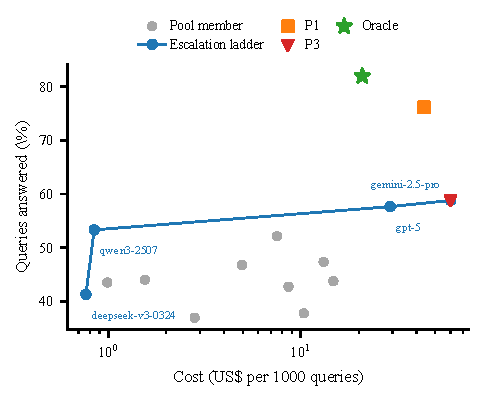
\includegraphics[width=\columnwidth]{figures/public_frontier}}
\caption{The thirteen models of the public pool, the cost--accuracy
frontier they define and where the escalation policies land on it. Cost is
logarithmic, in US dollars per 1{,}000 queries. P3 sits on the top rung it
always uses. P1 climbs the frontier and answers more queries than any
single model in the pool, at a price between the two costliest rungs. The
oracle answers still more for a third of what P3 costs.}
\label{fig:public-frontier}
\end{figure}

\begin{table*}[!t]
\caption{The public pool in cost order, over the 12{,}168 queries of nine
datasets that all thirteen models answered. Cost is the provider's own
charge, in US dollars per 1{,}000 queries. The $c^*$ share is the fraction
of queries for which that model is the cheapest one that answers
correctly, and the last row the queries no model answers. A bullet marks
the four models on the cost--accuracy frontier, which are the rungs of the
escalation ladder.}
\label{tab:public-pool}
\centering
\generated{tables/public_pool.tex}{\setlength{\tabcolsep}{4pt}
\begin{tabular}{@{}lrrrrc@{}}
\toprule
Model & Acc.\ (\%) & Cost (\$/1{,}000) & \$ per solved (/1{,}000) & $c^*$ share (\%) & Ladder \\
\midrule
\texttt{deepseek-v3-0324} & 41.3 & 0.76 & 1.85 & 7.1 & $\bullet$ \\
\texttt{qwen3-235b-a22b-2507} & 53.3 & 0.84 & 1.58 & 39.4 & $\bullet$ \\
\texttt{deepseek-v3.1-terminus} & 43.5 & 0.99 & 2.27 & 9.6 &  \\
\texttt{kimi-k2-0905} & 44.0 & 1.55 & 3.52 & 4.0 &  \\
\texttt{intern-s1} & 36.9 & 2.81 & 7.61 & 1.9 &  \\
\texttt{gpt-5-chat} & 46.8 & 4.95 & 10.59 & 3.4 &  \\
\texttt{qwen3-235b-a22b-thinking-2507} & 52.1 & 7.52 & 14.43 & 1.5 &  \\
\texttt{gemini-2.5-flash} & 42.7 & 8.63 & 20.23 & 5.7 &  \\
\texttt{claude-sonnet-4} & 37.7 & 10.36 & 27.47 & 0.5 &  \\
\texttt{deepseek-r1-0528} & 47.3 & 13.14 & 27.77 & 1.5 &  \\
\texttt{glm-4.6} & 43.7 & 14.78 & 33.78 & 1.6 &  \\
\texttt{gpt-5} & 57.6 & 29.15 & 50.57 & 3.4 & $\bullet$ \\
\texttt{gemini-2.5-pro} & 58.8 & 60.02 & 102.08 & 2.4 & $\bullet$ \\
\midrule
No model answers & -- & -- & -- & 18.0 &  \\
\bottomrule
\end{tabular}
}
\end{table*}

\begin{table*}[!t]
\caption{Escalation policies on the public pool under oracle detection, in
US dollars per 1{,}000 queries. P1 climbs the cost--accuracy frontier, P3
uses its top rung once, P4 starts uniformly over the pool and then climbs,
and Random picks a model uniformly and recovers at the top rung. A policy
that answers fewer queries can show a negative tax, underpaying by
failing, so the tax is read beside the solved column.}
\label{tab:public-tax}
\centering
\generated{tables/public_tax.tex}{\setlength{\tabcolsep}{4pt}
\begin{tabular}{@{}lrrrrr@{}}
\toprule
Policy & Solved (\%) & Attempts & Cost (\$/1{,}000) [95\% CI] & Tax [95\% CI] & Tax / $c^*$ cost \\
\midrule
P1, climb the frontier & 76.2 & 2.27 & 43.73 [41.98, 45.54] & 16.12 [15.11, 17.17] & 2.69 \\
P3, sticky top & 58.8 & 1.00 & 60.02 [58.62, 61.41] & 47.74 [46.41, 49.04] & 7.96 \\
P4, uniform start & 71.0 & 1.83 & 54.03 [52.34, 55.77] & 28.28 [27.25, 29.29] & 4.72 \\
Random, then top & 64.5 & 1.50 & 47.22 [45.82, 48.61] & 29.48 [28.44, 30.51] & 4.92 \\
\midrule
Always \texttt{deepseek-v3-0324} & 41.3 & 1.00 & 0.76 [0.74, 0.79] & -5.31 [-5.86, -4.78] & -0.89 \\
Always \texttt{qwen3-235b-a22b-2507} & 53.3 & 1.00 & 0.84 [0.81, 0.87] & -5.27 [-5.82, -4.75] & -0.88 \\
Always \texttt{gpt-5} & 57.6 & 1.00 & 29.15 [28.31, 30.01] & 18.34 [17.69, 19.01] & 3.06 \\
Always \texttt{gemini-2.5-pro} & 58.8 & 1.00 & 60.02 [58.62, 61.41] & 47.74 [46.41, 49.04] & 7.96 \\
\midrule
Oracle & 82.0 & 1.00 & 20.88 [19.84, 21.96] & 0.00 [0.00, 0.00] & 0.00 \\
\bottomrule
\end{tabular}
}
\end{table*}

The local grid stops at 8B parameters. Section~\ref{sec:public-arm}
recomputes the same quantities on the published outcomes of
LLMRouterBench: thirteen flagship models, nine datasets and 12{,}168
queries every model answered, priced by the providers themselves.

Table~\ref{tab:public-pool} and Fig.~\ref{fig:public-frontier} give the
pool in cost order. Its members span
a factor of 79 in price, from \$0.76 to \$60.02 per thousand queries, and
a factor of 1.6 in accuracy, from 36.9\% to 58.8\%. Price and accuracy are
only loosely related: of the eleven models dearer than
\texttt{qwen3-235b-a22b-2507}, nine answer fewer queries than it does. Only
four of the thirteen lie on the cost--accuracy frontier, and those four
are the ladder a rational escalator would climb. Between them the thirteen
answer 82.0\% of the queries; the remaining 18.0\% are beyond the pool.
The distribution of the minimum sufficient model repeats what the local
grid shows: the two cheapest models are the cheapest sufficient choice for
46.5\% of all queries, and the costliest model is that choice for 2.4\%.
Another 29.8\% are answered most cheaply by a model off the frontier,
which matters for what follows.

Table~\ref{tab:public-tax} gives the policies. Sticky use of the top of
the ladder (P3) costs 7.96 times the minimum sufficient cost, close to the
local grid's figure, and answers 58.8\% of queries. Climbing the frontier
(P1) costs 2.69 times, answers 76.2\% and takes 2.27 attempts per query.
The oracle answers 82.0\% at \$20.88 per thousand queries. Per solved
query the ordering is the same and the comparison is fair across policies
of unequal success: \$25.47 for the oracle, \$57.38 for P1 and \$102.08
for P3, so a user who always reaches for the strongest model pays four
times what a perfect one-shot router would pay for the same answers.

Two features of the pool are worth separating from the local grid. First,
the frontier is a subset: a policy climbing it fails on queries only an
off-frontier model answers, and then pays four cheap attempts instead of
one expensive sufficient model. This is why the two cheapest static
policies show a negative tax, and why on SimpleQA even P1 does; they
underpay by failing, answering 41.3\% and 53.3\% of queries. Tax is
meaningful only beside the success rate, which is why cost per solved
query carries the comparison. Second, the dollar tax is larger than the
token tax --- 7.96 against 2.04 for P3 --- because the price per token
spans two orders of magnitude across providers while the answers
themselves do not differ in length nearly as much. Escalation on a mixed
pool is expensive in a way that token counts hide.

The thinking and non-thinking releases of Qwen3-235B-A22B give the public
counterpart of the mode axis. Thinking costs 9.11 times more per solved
query [8.78, 9.47] and, over all nine datasets, answers slightly fewer
queries (52.1\% against 53.3\%). The plain release already answers 53.3\%
of queries on its own and only 9.3\% need thinking, so the mode is worth
paying for on a small minority of queries and is picked per query or not
at all. Where reasoning is the point the picture reverses --- on GPQA
thinking answers 80.3\% against 58.6\% --- which is the same
family-dependence the local grid shows.

Scoring a judged Arena-Hard tie as half credit rather than requiring a
full score moves nothing: P3 pays 8.14 times the minimum sufficient cost
and P1 2.64 times, against 7.96 and 2.69.

\subsection{The Escalation Tax on a Hosted Frontier Ladder}
\label{sec:results-hosted}

\begin{figure}[!t]
\centering
\generated{figures/hosted_frontier.pdf}
{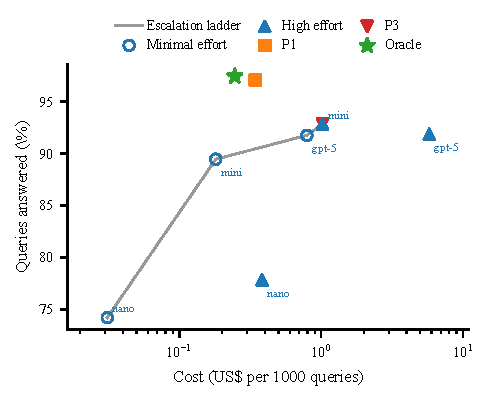
\includegraphics[width=\columnwidth]{figures/hosted_frontier}}
\caption{The six hosted cells on the cost--accuracy plane, open for
minimal reasoning effort and filled for high. Cost is logarithmic, in US
dollars per 1{,}000 queries. The grey line is the frontier the escalation
policies climb. The mode axis reads as the horizontal step from an open
marker to the filled marker of the same model.}
\label{fig:hosted-frontier}
\end{figure}

\begin{table*}[!t]
\caption{The six hosted cells: three model sizes crossed with two
reasoning efforts, on the prompts of the local main subset. Output tokens
include reasoning tokens, which the provider reports separately but bills
as output. A cap hit is a truncated generation, counted as a failure
exactly as a local cap hit is.}
\label{tab:hosted-cells}
\centering
\generated{tables/hosted_cells.tex}{\setlength{\tabcolsep}{3pt}
\begin{tabular}{@{}lllrrrrrr@{}}
\toprule
Cell & Model & Effort & Cap & Acc.\ (\%) & Out.\ tok. & Reas.\ tok. & Cap hit (\%) & Cost (\$/1{,}000) \\
\midrule
$h_1$ & \texttt{gpt-5-nano} & Minimal & 2{,}048 & 62.5 & 108 & 0 & 0.0 & 0.02 \\
$h_2$ & \texttt{gpt-5-nano} & High & 4{,}096 & 85.0 & 1{,}738 & 1{,}664 & 12.5 & 0.35 \\
$h_3$ & \texttt{gpt-5-mini} & Minimal & 2{,}048 & 97.5 & 147 & 0 & 0.0 & 0.16 \\
$h_4$ & \texttt{gpt-5-mini} & High & 4{,}096 & 97.5 & 824 & 675 & 0.0 & 0.84 \\
$h_5$ & \texttt{gpt-5} & Minimal & 2{,}048 & 100.0 & 132 & 0 & 0.0 & 0.73 \\
$h_6$ & \texttt{gpt-5} & High & 4{,}096 & 100.0 & 887 & 760 & 0.0 & 4.50 \\
\bottomrule
\end{tabular}
}
\end{table*}

\begin{table*}[!t]
\caption{Escalation policies on the hosted ladder under oracle detection,
in US dollars per 1{,}000 queries. The static rows are the ladder rungs
used alone. As on the public pool, a policy that answers fewer queries can
show a negative tax by underpaying through failure, so the tax is read
beside the solved column.}
\label{tab:hosted-tax}
\centering
\generated{tables/hosted_tax.tex}{\setlength{\tabcolsep}{4pt}
\begin{tabular}{@{}lrrrrr@{}}
\toprule
Policy & Solved (\%) & Attempts & Cost (\$/1{,}000) [95\% CI] & Tax [95\% CI] & Tax / $c^*$ cost \\
\midrule
P1, climb the frontier & 100.0 & 1.40 & 0.08 [0.05, 0.14] & 0.02 [0.00, 0.06] & 0.34 \\
P3, sticky top & 100.0 & 1.00 & 0.73 [0.57, 0.90] & 0.66 [0.51, 0.83] & 10.60 \\
P4, uniform start & 99.6 & 1.10 & 1.15 [0.85, 1.49] & 1.09 [0.79, 1.42] & 17.41 \\
Random, then top & 100.0 & 1.10 & 1.18 [0.87, 1.51] & 1.11 [0.82, 1.44] & 17.81 \\
\midrule
Always $h_{1}$ & 62.5 & 1.00 & 0.02 [0.02, 0.03] & -0.04 [-0.06, -0.02] & -0.61 \\
Always $h_{3}$ & 97.5 & 1.00 & 0.16 [0.12, 0.21] & 0.10 [0.06, 0.14] & 1.57 \\
Always $h_{5}$ & 100.0 & 1.00 & 0.73 [0.57, 0.90] & 0.66 [0.51, 0.83] & 10.60 \\
\midrule
Oracle & 100.0 & 1.00 & 0.06 [0.05, 0.08] & 0.00 [0.00, 0.00] & 0.00 \\
\bottomrule
\end{tabular}
}
\end{table*}

\tbd{Written when the hosted main stage finishes: the ladder and where
high effort falls off it, the $c^*$ distribution against the local
grid's, the policy taxes, and the reasoning-token cost of the mode axis.}

\subsection{Carbon of the Escalation Tax}
\label{sec:results-carbon}

\begin{table}[!t]
\caption{Carbon of the escalation tax under oracle detection, in grams of
CO$_2$e per 1{,}000 queries. The kWh column is the policy's own energy for
those queries; every carbon figure follows from it by multiplication. The
four columns are grid carbon intensities in gCO$_2$e/kWh: 50 for a grid
carried by nuclear or hydro, 250 for a large renewable share, 475 for the
figure usually quoted as the global average, and 700 for a grid carried by
coal. They are round values spanning the range grids occupy, not
measurements of a named region.}
\label{tab:carbon}
\centering
\generated{tables/carbon.tex}{\begin{tabular}{@{}lrrrrr@{}}
\toprule
Policy & kWh & 50 & 250 & 475 & 700 \\
\midrule
P1, frugal climb & 0.242 & 2.35 & 11.76 & 22.35 & 32.93 \\
P2, think first & 0.719 & 22.94 & 114.70 & 217.93 & 321.16 \\
P3, sticky high & 0.800 & 34.31 & 171.57 & 325.99 & 480.40 \\
P4, uniform start & 0.438 & 12.71 & 63.55 & 120.74 & 177.94 \\
P4, start skewed to $c_8$ & 0.593 & 21.97 & 109.84 & 208.71 & 307.57 \\
Random, then $c_8$ & 0.585 & 21.60 & 108.01 & 205.22 & 302.43 \\
Oracle & 0.164 & 0.00 & 0.00 & 0.00 & 0.00 \\
\bottomrule
\end{tabular}
}
\end{table}

\tbd{Written with the local energy results: the tax in carbon terms, and
whether the bracket is wide enough to reorder the policies.}

% =====================================================================
%  VI. DISCUSSION  --  STUB
%  Planned content:
%    A. Why the observed effects occur, including failure cases.
%    B. Limitations, stated plainly:
%       - all cells are Q4_K_M quantised models; size comparisons are
%         between quantised models
%       - the largest cell is 8B; frontier tiers may behave differently
%         (addressed in part by the public-benchmark arm)
%       - escalation policies are constructed, not observed
%       - one machine and one GPU; energy figures do not transfer to other
%         silicon and are not claimed to
%       - labels depend on the generation caps (gate 2, finding 2)
%       - judge validity for the open-ended family
%    C. Implications for providers and for users.
% =====================================================================
\section{Discussion}
\label{sec:discussion}

\tbd{Section to be written once results exist.}

% =====================================================================
%  VII. FUTURE SCOPE
%  The directions below follow from the design and its limitations
%  (Section VI-B). Directions that depend on the results are added, and
%  any of these that the results undercut are dropped, once Section V
%  exists.
% =====================================================================
\section{Future Scope}
\label{sec:future}

Several directions follow from the limitations in
Section~\ref{sec:limitations}.

\emph{Observing escalation.} The constructed policies and the swept
detection probabilities are the least grounded part of the comparator. A
study that records how people move between the configurations of a tiered
service, including where they start, how often they notice a wrong answer
and when they give up, would replace those assumptions with estimates. It
would turn the computed tax into a measured one and give P4 an observed
starting distribution.

\emph{Continuous reasoning budgets.} Qwen3 and several hosted services let
the amount of reasoning be set as a token budget or an effort level rather
than switched on or off. Treating the budget as a continuous axis would turn
the eight-cell grid into a surface, and the router's decision into a choice
of size and budget. The dependence of our labels on the thinking cap points
the same way, since the cap is a budget fixed once for every prompt.

\emph{Conversations and switching costs.} A cost model in which a retry
carries the conversation so far, and in which moving to another size pays
for loading it, would bring the tax closer to what users of memory-limited
hardware pay. It would also make the best choice for a query depend on the
model already loaded, which a one-shot router of the kind studied here does
not consider.

\emph{Routing the wider pools.} The public and hosted arms show what the tax
costs on pools that mix model families and frontier tiers, but both report
manual policies and the oracle rather than a trained router. Adding one
means recovering each public query's text from its source dataset and
training on outcomes we did not generate, or paying to label enough hosted
prompts to train on. Doing either, and adding quantisation as a third axis
beside size and mode, would test whether the minimum sufficient
configuration can still be predicted when cells differ in more than size and
mode.

\emph{Whole-system energy.} Measuring processor and memory power alongside
the GPU would close the energy boundary, and it would give CPU routers a
measured cost in place of an upper bound.

\emph{Online adaptation.} Providers change models and prices, and a router
trained on one pool's labels goes stale. The outcomes of routed queries,
as revealed by whether the user accepts an answer or retries, could keep a
router current without relabelling every prompt in every cell. That is a
partial-feedback problem, because only the routed cell's outcome is ever
observed.

\tbd{Add directions motivated by the results, and drop any of the above
that the results undercut, once Section~\ref{sec:results} exists.}


\bibliographystyle{IEEEtran}
\bibliography{refs,refs-methods}

\begin{IEEEbiographynophoto}{Indrajeet Mondal}
\decision{author biography, with a photograph 1\,in wide by 1.25\,in tall;
one entry per author}
\end{IEEEbiographynophoto}

\EOD

\end{document}
